\section{Formato de mensajes}
Los mensajes enviados entre los nodos deben tener un formato compatible con las
redes CAN convencionales. Por ello el mensaje tiene un tamaño que varía desde
los 44 bytes hasta los 108 bytes, dependiendo de la cantidad de datos en el
\textit{Data Field}.

En la Figura \ref{fig:Data_Frame} se observa la el formato de Frame de datos de
los mensajes CANae.

\begin{figure}[h!]
 \centering
 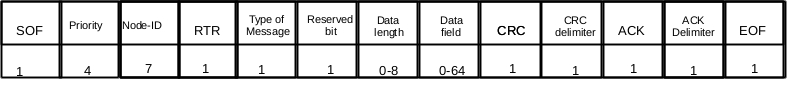
\includegraphics[scale=0.6]{images/Secciones/AppendixA/Data_Frame.jpg}
  \caption{Frame de datos CANae}
\label{fig:Data_Frame}
\end{figure}

Los campos del mensaje son los siguientes:

\begin{itemize}
\item Start of Frame (SOF) - 1 bit: Este bit marca el comienzo de un frame.
  Suele ser 0.
\item Priority - 4 bits: Este campo declara la prioridad del frame. 
\item Node-ID - 7 bits: El ID del Nodo origen.
\item Remote transmission request (RTR) - 1 bit: Bit dominante (0) para frames
  de datos o eventos, y bit recesivo (1) para frames remotos. Un frame remoto
  es un mensaje que es enviado en forma automática por algun sensor. Los frames
  remotos se utilizan para enviar telemetría por parte de los sensores y
  componentes.
\item Type of Message (TOM) - 1 bit: Bit dominante (0) si es un evento, y bit
  recesivo (1) para frames remotos.
\item Bit reservado - 1 bit: Este bit está reservado para futuras aplicaciones.
  En esta versión debe ser un bit dominante (0).
\item Data length - 0-4 bytes: Cantidad de bytes del campo de datos.
\item Data field - 0-64 bytes: Datos.
\item CRC - 15 bits: Cyclic redundancy check.
\item CRC delimier - 1 bit: Debe ser recesivo (1).
\item ACK - 1 bit: El transmisor debe poner este bit en recesivo (1), y el
  receptor puede responder este bit con un bit dominante (0).
\item ACK delimiter: Debe ser recesivo (1).
\item End-of-Frame (EOF) - 7 bits: Final del frame de datos.
\end{itemize}

El Data field tiene el siguiente formato: el primer byte siempre es el ID de la
función, evento y/o comando. Esto significa que es posible definir un número de
$2^8 = 256$ funciones, eventos y comandos diferentes.

Los siguientes bytes (del 1 al 63) son argumentos de las funciones o datos.

Debe entenderse que esto no es mandatorio, ya que se pueden definir ID de
dos o más bytes reduciendo la cantidad de datos. 
